%% LyX 2.2.1 created this file.  For more info, see http://www.lyx.org/.
%% Do not edit unless you really know what you are doing.
\documentclass[english,brazil,oldfontcommands]{abntex2}
\usepackage[T1]{fontenc}
\usepackage[utf8]{inputenc}
\usepackage{array}
\usepackage{refstyle}
\usepackage{float}
\usepackage{booktabs}
\usepackage{multirow}
\usepackage{amsmath}
\usepackage{graphicx}
\usepackage{nomencl}
% the following is useful when we have the old nomencl.sty package
\providecommand{\printnomenclature}{\printglossary}
\providecommand{\makenomenclature}{\makeglossary}
\makenomenclature

\makeatletter

%%%%%%%%%%%%%%%%%%%%%%%%%%%%%% LyX specific LaTeX commands.
%% Because html converters don't know tabularnewline
\providecommand{\tabularnewline}{\\}
\RS@ifundefined{subsecref}
  {\newref{subsec}{name = \RSsectxt}}
  {}
\RS@ifundefined{thmref}
  {\def\RSthmtxt{theorem~}\newref{thm}{name = \RSthmtxt}}
  {}
\RS@ifundefined{lemref}
  {\def\RSlemtxt{lemma~}\newref{lem}{name = \RSlemtxt}}
  {}


%%%%%%%%%%%%%%%%%%%%%%%%%%%%%% Textclass specific LaTeX commands.
% adaptação do suporte ao natbib do LyX para uso do abntex2cite
\AtBeginDocument{%                % garante que este código será carregado após
% \usepackage[alf]{abntex2cite} ou
% \usepackage[num]{abntex2cite}
% no preâmbulo latex.
\RequirePackage{abntex2cite}   % previne o não carregamento do abntex2cite,
% mas não define se as citações serão do
% tipo 'alf' ou 'num'.
\renewcommand{\citeauthor}[1]{\citeauthoronline{#1}}
\def\citep{\cite}
\newcommand{\citeyearpar}[1]{(\citeyear{#1})}
\ifx\AbntCitetype\AbntCitetypeALF
\def\citet{\citeonline} % alf
\newcommand{\citealt}[1]{\citeauthoronline{#1}~\citeyear{#1}}
\newcommand{\citealp}[1]{\citeauthoronline{#1},~\citeyear{#1}}
\else
\def\citet{\@ifnextchar[{\citet@with}{\citet@without}} % num
\def\citet@with[#1]#2{\citeauthoronline{#2}~\cite[#1]{#2}}
\def\citet@without#1{\citeauthoronline{#1}~\cite{#1}}
\newcommand{\citealt}[1]{\citeauthoronline{#1}~\citeonline{#1}}
\def\citealp{\citeonline}
\fi
}

%%%%%%%%%%%%%%%%%%%%%%%%%%%%%% User specified LaTeX commands.
\usepackage{fncychap}
\makechapterstyle{icmc}{%
   % Secao secundaria (Section) Caixa baixa, Negrito
    \renewcommand*{\cftsectionfont}{\bfseries}
    % Secao terciaria (Subsection) Caixa baixa, Negrito, italico
    \renewcommand*{\cftsubsectionfont}{\itshape\bfseries}
    % Secao quaternaria (Subsubsection) Caixa baixa, italico
    \renewcommand*{\cftsubsubsectionfont}{\itshape}
    % Secao quinquenária (Subsubsubsection) Caixa baixa
    \renewcommand*{\cftparagraphfont}{\normalsize}

   % tamanhos de fontes de chapter e part	
   \ifthenelse{\equal{\ABNTEXisarticle}{true}}{%
     \setlength\beforechapskip{\baselineskip}
     \renewcommand{\chaptitlefont}{\ABNTEXsectionfont\ABNTEXsectionfontsize}
    }{%else
     \setlength{\beforechapskip}{0pt}
     \renewcommand{\ABNTEXchapterfontsize}{\LARGE}
    
    %\renewcommand{\ABNTEXchapterfont}{\sffamily\bfseries}  %alteração da fonte dos capítulos, seções e subseções
    \renewcommand{\chaptitlefont}    {\ABNTEXchapterfont\bfseries\ABNTEXchapterfontsize}
  

% impressao do numero do capitulo
  \renewcommand{\chapternamenum}{}
  
  % impressao do nome do capitulo
  \renewcommand{\printchaptername}{%
   %\chaptitlefont
   %\ifthenelse{\boolean{abntex@apendiceousecao}}{\appendixname}{\chaptername}%
  }
% impressao do titulo do capitulo
  \def\printchaptertitle##1{%
    
    \setboolean{ABNTEXupperchapter}{true}
    
    \ifthenelse{\boolean{abntex@innonumchapter}}{
        \vskip 0ex \hrulefill\chaptitlefont\bfseries\ABNTEXchapterupperifneeded{##1}
        \vskip -0.6ex\hfill\rule{.8\textwidth}{0.5pt} 
        \vskip -2.8ex\hfill\rule{.8\textwidth}{2pt}
        \vskip 1.5ex
    
    }{%
    % else
        {\hrulefill
        {\renewcommand{\arraystretch}{1.5} %  1 is the default, change whatever you need
        \begin{tabular}{|c|}
            \rowcolor{black}\color{white}\normalsize\ABNTEXchapterfont
              \ifthenelse{\boolean{abntex@apendiceousecao}}{\MakeTextUppercase{\appendixname}}{\MakeTextUppercase{\chaptername}}  \\ 
            \vspace{-1.5ex}\\ %coloquei para aumentar o espaço entre o título e o número
            \resizebox{!}{1.1cm}{\ABNTEXchapterfont\thechapter}
            \\[2.5ex]
            \hline
        \end{tabular}}} \\
        \vskip 4.3ex \flushright\chaptitlefont\bfseries\ABNTEXchapterupperifneeded{##1} \\
        \vskip -0.6ex\hfill\rule{.8\textwidth}{0.5pt} \\
        \vskip -2.8ex\hfill\rule{.8\textwidth}{2pt}\\
        \vskip 1.5ex
}    
        
  }
       


 }

}
\chapterstyle{icmc}

\makeatother

\usepackage{babel}
\begin{document}
A Informática Biomédica tem sido, ao longo das últimas décadas, um
campo emergente graças aos progressos feitos nos campos da computação,
microeletrônica e telecomunicações. No entanto, ainda não existe uma
definição universal para “Informática” nos campos da medicina. A Informática
Biomédica pode ser considerada como a ciência da informação aplicada
no estudo do contexto da biomedicina, que surgiu para atender as aplicações
da TI (Tecnologia da Informação) na área da saúde \citep{Bulu}. Por
sua vez, a Informática Radiológica (sub\nobreakdash-área da informática
biomédica) é a área da radiologia responsável pela melhoria da eficiência,
precisão e confiabilidade dos serviços radiológicos dentro da área
médica \citep{Serique2012}. 

Embora em radiologia muitas coisas, incluindo a criação da imagem,
sejam bastante padronizadas, existem muitas maneiras de se descrever
o conteúdo de uma imagem, incluindo diferentes sinônimos de termos,
vários níveis de descrição e foco em atores diferentes. Nesse contexto,
o uso de terminologias visuais e estruturadas para anotações em imagens
é uma abordagem promissora, pois permite a definição precisa de imagens
médicas utilizando a semântica fornecida pelas anotações \citep{Channin2010}.

Atualmente, anotações sobre imagens médicas fornecem apenas algumas
informações, como, por exemplo, metadados que contém o nome do paciente,
idade, médico responsável, etc. As imagens em si não possuem nenhuma
informação semântica, por isso, essas anotações não podem ser automaticamente
integrados em aplicações médicas avançadas, tais como aquelas para
o apoio à decisão clínica. Para facilitar o processamento dessas anotações
por máquina, é necessário adicionar informações semânticas que sejam
baseadas em fontes de conhecimento, como \foreignlanguage{english}{sistemas
de\emph{ staging}}. Além disso, é preciso que essas informações sejam
codificadas de forma compreensíveis para maquinas, utilizando-se ontologias
para facilitar o mapeamento entre conceitos semânticos. Assim, será
possível a realização de um processamento mais complexo, como por
exemplo, o uso\emph{ de reasoning} \citep{Dasmahapatra}.

Como o foco deste trabalho é um sistema de classificação automática
de pacientes con câncer a partir de imagens usando \textit{reasoning}
baseados em sistemas de notação como TNM. Este capítulo abordará os
principais conceitos referentes a Sistemas de suporte à decisão assistido
por computador, em seguida, na seção 2.2 Informática Radiológica,
em seguida, na Seção 2.2, Imagens Medicas. Na seção 2.3, é discutido
o processo de Anotações em imagens. Por fim, na seção 2.4, serão descritos
os sistemas de \emph{staging} que são a base de conhecimento para
a classificação dos pacientes com câncer, a partir de imagens radiológicas.

\section{Informática Biomédica para sistemas de suporte à decisão assistido
por computador}

Nao é que até os anos 70 que os sistemas de suporte à decisão influenciadas
pela informática biomédica foram vistos. Trabalhos como \citep{dombal}
com seu sistema chamado INTERNIST-I e \citep{Myers:1987:BII:41526.41543}
que desenvolveu um sistema baseado en regras para diagnóstico, representam
desenvolvimentos iniciais importantes de sistemas de informática biomédica
\citeonline{pmid23431259}. Mais tarde houve toda uma evolução significativa
com grande reconhecimento de seu sucesso na melhoria de desempenho
destos sistemas, que é descrito por \citep{Pearson2009}. Esta evolução
permitiu o nascimento de mais subgêneros específicos de métodos de
informática biomédica e suas implementações na forma de sistemas de
diagnóstico assistido por computador. Nesse contexto o apoio à decisão
na prática radiológica clínica faz a sua aparição \citep{Stivaros}.

há uma série de áreas de aplicação na medicina para que os sistemas
de apoio à decisão auxiliada por computador tornaram-se implementados.
Algumas das principais áreas de aplicação são : Medicina de Emergência
e Unidades de Terapia Intensiva, Medicina cardiovascular, Aplicações
dentárias, Medicina Pediátrica, Radiologia e Câncer.

No caso de câncer, a informática biomédica começou a desempenhar um
papel importante na detecção e tratamento do câncer, muitos estudos
aplicam metodos como redes neurales e sistemas híbridos através da
combinação de informações heterogêneas. O uso de ferramentas de diagnóstico
auxiliado por computador tem o potencial para reduzir a variabilidade
entre as opiniões de especialistas, bem como melhorar a precisão diagnóstica
para a interpretação do classificação de cancer \citep{Jiang}.

No caso de Radiologia, o processamento de imagem baseado em computador
é uma área de pesquisa ativa. O processamento de imagem combinado
com a visualização e aprendizagem de maquina para a tomada de decisões
tem proporcionado uma mais-valia para aplicações clínicas, e mais
recentemente com o surgimento de múltiplas tecnologias de imagens
médicas: como a tomografia computadorizada (CT), raios-X, ressonância
magnética (MRI), ressonância magnética funcional e (FMRI), numerosos
métodos biomédicos foram concebidos como soluções de aplicações clínicas
específicas.

A seguir, descreveremos as características de algumas dessas tecnologias
de imagens e sua aplicação no estudo de pacientes com câncer.

\section{Tecnologias para Imagens Médicas}

A pesquisa e tratamento do câncer são ambos criticamente dependentes
de tecnologias de imagens. Avanços em imagem já permitem uma precisão
notável em detectar se um tumor invadiu tecidos vitais, cresceu ou
se espalhou para órgãos distantes; permitindo que os médicos possam
monitorar o progresso do paciente sem a necessidade de biópsias ou
outros métodos invasivos \citep{Imaging2007}.

Antes de analisar como é que a semântica pode ser adicionada no processo
de monitoramento do progresso dos pacientes com câncer, é importante
compreender as tecnologias de imagem primárias com que iremos trabalhar
em nossa proposta e o que elas fazem. Essas tecnologias de imagem
abrangem \foreignlanguage{english}{Computed Tomography} (CT\nomenclature{CT}{Computed Tomography})
e \foreignlanguage{english}{Positron Emission Tomography} (PET\nomenclature{PET}{Positron Emission Tomography}). 

\subsection{Tomografia Computadorizada}

A tomografia computadorizada, ou \foreignlanguage{english}{Computed
Tomography} (CT), usa técnicas de reconstrução intensivas por computador
para criar imagens 3D do corpo a partir de raios-X. Devido ao uso
de computadores, uma gama de densidades mais elevada pode ser exibida
em comparação com imagens de raios-X convencionais. Esse recurso permite
a diferenciação entre órgãos e patologias e detectar a presença de
materiais específicos, tais como gordura ou cálcio. Assim como em
imagens convencionais de raios-X, objetos de alta densidade causam
mais atenuação e, portanto, são exibidos como cinza mais claro que
objetos de baixa densidade. 

Por exemplo, no CT do peito uma vasta gama de densidades de tecido
está presente, uma boa imagem das estruturas do mediastino são mostradas
em detalhes do pulmão, mostrados na Figura \ref{fig:CT1}.

Tomografias estão entre as tecnologias de imagem mais comuns utilizados
no diagnóstico, bem como no planejamento e monitoramento do tratamento
de câncer; especialmente na detecção de câncer de fígado, pâncreas,
pulmões e ossos\citep{Imaging2007}. 

\begin{figure}
\caption{CT do peito, (a) anatomia do mediastino: Átrio direito (RA), Ventrículo
direito (RV), Válvula aórtica (AV), Aorta (A), Átrio esquerdo (LA).
(b) Anatomia do pulmão.\label{fig:CT1}}

\noindent \begin{centering}
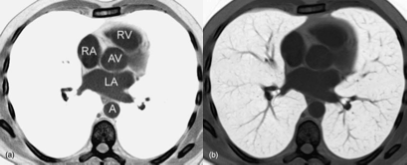
\includegraphics[width=0.7\columnwidth]{../figures/CTjoin}
\par\end{centering}
\fadaptada{Arnold2012}
\end{figure}

\selectlanguage{english}%

\subsection{Positron Emission Tomography}

\selectlanguage{brazil}%
Os exames de \foreignlanguage{english}{Positron Emission Tomography}
(PET) fornecem uma ferramenta fundamental na gestão e terapia de câncer
para muitos tumores comuns. A maioria dos estudos clínicos de PET
são realizados para determinar o grau de um tumor, a localização e
número de metástases. 

Nesses estudos oncológicos PET, o paciente recebe uma injecção do
açúcar radioactivo que pode ajudar na localização de um tumor, porque
as células cancerosas  utilizam o azucar (glicose) mais avidamente
do que outros tecidos no corpo\citep{ZIEGLER2005679}. 

Por exemplo, a Figura \ref{fig:METASTA} mostra um exemplo de um paciente
com metástases de câncer de cólon, onde a glicose no tecido canceroso
é facilmente visível. Por esse motivo, para muitos tumores comuns,
a PET é a técnica mais precisa para visualizar a propagação do tumor
ou a sua resposta à terapia\citep{Imaging2007}. 

\begin{figure}
\caption{Estudo de paciente com metástase de cólon, pode ser visto que o aumento
da captação de glicose no tecido canceroso é facilmente visível. \label{fig:METASTA}}

\noindent \begin{centering}
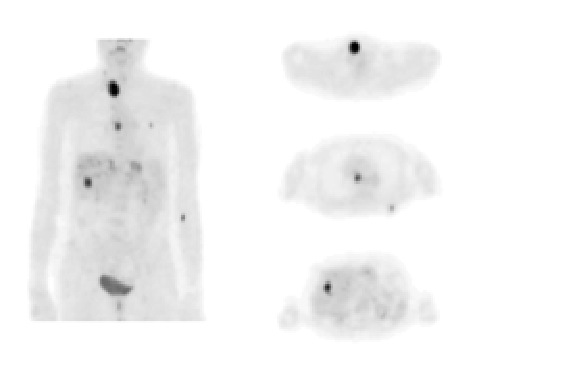
\includegraphics{../figures/metastases}
\par\end{centering}
\fadaptada{ZIEGLER2005679}
\end{figure}

É bom notar que, o sistema ePAD no qual vamos desenvolver nossa proposta,
permite a manipulação de imagens de TC e PET\citep{Rubin2014}.

Todas as modalidades de análise acima mencionadas fornecem uma visão
detalhada sobre a anatomia humana, suas funções, associações a doenças.
As técnicas avançadas de análise dessas imagens geram parâmetros quantitativos
adicionais, abrindo assim o caminho para a melhoria da prática clínica
e diagnóstico\citep{Zillner2013}. 

Embora imagens não processadas (raw images) possam ser úteis em algumas
aplicações de processamento por computador, grande parte do conteúdo
semântico nas imagens e dos relatórios radiológicos associados a elas,
não é explícito ou disponível para computadores. Isso dificulta a
descoberta de novas informações num grande volume de informação. Com
base nisso, as aplicações médicas avançadas devem possuir descrições
semânticas sobre dados clínicos, dados como as imagens medicas.

\section{Anotação de Imagens }

A necessidade de anotar imagens é reconhecida em uma ampla variedade
de aplicações diferentes, abrangendo tanto o uso profissional e pessoal
de dados sobre imagens. Anotação de imagens é uma tarefa complexa,
que tem sido amplamente estudada nos domínios da visão computacional
e recuperação de imagens. 

No contexto da radiologia, anotar imagens é uma tarefa que pode ser
assistido por computador. No entanto, os radiologistas geralmente
não gravam suas anotações num formato estruturado, que seja acessível
por máquina, impedindo assim o bom desempenho dos sistemas de decisão
sobre diagnósticos. O desempenho deste tipo de sistema baseia-se na
escolha dos termos que estão sendo usados para descrever o conteúdo
das imagens. Essa escolha é altamente dependente da aplicação, as
necessidades e a experiência do usuário.

Tais termos podem ser diretamente derivados da terminologia fornecida
pelos radiologistas em seus relatórios ou automaticamente previsto
a partir das características das imagens \citep{Gimenez2011}. Eles
podem ser usados para descrever uma variedade de informações sobre
o conteúdo de uma imagem (por exemplo, a forma da lesão de um tumor
canceroso). Esses termos podem representar também o conteúdo semântico
da imagem, nesse caso eles podem ser chamados de anotações semânticas. 

As anotações semânticas estão diretamente ligados ao alto nível de
compreensão e descrições do usuário sobre as características da imagem
\citep{Rubin2011}. Com base nessas considerações, incorporar características
semânticas em sistemas de decisão sobre diagnóstico pode ser uma tentativa
promissora para preencher a lacuna semântica entre a descrição visual
de uma imagem e seu significado \citep{Ma2010}, Figura \ref{AnnotaimagemCT}.

\begin{figure}
\caption{A imagem CT do fígado anotada com termos semânticos. \label{AnnotaimagemCT}}

\noindent \begin{centering}
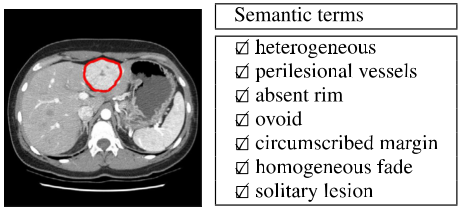
\includegraphics[width=0.8\columnwidth]{../figures/imageannotation}
\par\end{centering}
\fadaptada{Kurtz20141082}
\end{figure}


\subsection{Anotação Semântica}

De acordo com \citet{Nagarajan2006}, anotação é o processo de associar
metadados a recursos como áudio, vídeo, texto estruturado, páginas
web, imagens, etc. Enquanto que anotação semântica é o processo de
marcar com recursos de metadados semânticos. No contexto da biomedicina.
esse processo é conhecido como: anotação semântica de imagens médicas. 

Em radiologia, o processo de marcar imagens é um trabalho manual,
lento e inconsistente devido ao grande número de imagens que são geradas
por dia em hospitais modernos \citep{Depeursinge2014}. É por essa
razão que várias abordagens para enfrentar o desafio da anotação semântica
de imagens médicas já foram estudados. Por exemplo, em \citet{Moller2009}
uma abordagem para a extração de informações de \emph{DICOM }\foreignlanguage{english}{\emph{headers}}
e de relatórios estruturados\emph{ }DICOM\nomenclature{DICOM}{ Digital Imaging and Communications in Medicine}
(\foreignlanguage{english}{Digital Imaging and Communications in Medicine})
foi apresentada, \citet{seifer2009} introduziram um novo método para
a análise automática de imagens (em anatomia e com detetores de tecidos
específicos). Em outra frente, \citet{Rubin2008} integraram a anotação
manual de imagens no fluxo de trabalho dos radiologistas e\citet{Dasmahapatra}
introduziram uma abordagem de anotação de imagens para melhorar o
diagnóstico do câncer da mama. Todas essas abordagens fizeram uma
contribuição importante para melhorar o acesso às informações em imagens
médicas, especificando a \textquotedbl{}semântica'' das regiões nas
imagens. 

\subsection{Anotação de Imagens Médicas com Vocabulários Estruturados}

Embora o processo de descrição de imagens médicas utilizando conteúdo
semântico possa melhorar o acesso à informação médica, ele pode levar
a se ter diferentes descrições para uma mesma imagem. Isso prejudica
o bom desempenho de sistemas baseados nessas descrições, como por
exemplo os sistemas de apoio à decisão de diagnóstico. Para lidar
com esse problema, os últimos trabalhos no domínio semântico usam
vocabulários controlados para anotar as imagens \citep{Korenblum2011}.

Um vocabulário controlado fornece um conjunto de termos pré-definidos
para descrever características em imagens médicas. Esses vocabulários
podem facilitar a anotação de grandes conjuntos de imagens. Trabalhos,
como \citep{Napel2010}, investigaram métodos assistidos por computador
no apoio ao diagnóstico. Os autores utilizaram um banco de dados de
imagens onde as imagens foram anotadas semanticamente. O resultado
do estudo indicam que as anotações semânticas, usando um vocabulário
controlado, podem levar a diagnósticos mais precisos.
\selectlanguage{english}%

\section{Medical Background Knowledge}

\selectlanguage{brazil}%
Embora os vocabulários são os blocos de construção básicos para a
inferência sobre as técnicas de Web Semântica. Não há uma divisão
clara entre o que é referido como \textquotedbl{}vocabulários controlados\textquotedbl{}
e \textquotedbl{}ontologias\textquotedbl{}. Considerando que o vocabulário
é usado quando o formalismo rigoroso não é necessariamente usado ou
apenas em um sentido muito solto, podemos dizer que a diferença fundamental
entre uma ontologia e um vocabulário controlado é o nível de abstração
e relações entre conceitos.

As ontologias são vocabulários controlados expresso em uma linguagem
de representação de ontologias (como OWL) \citep{browne2004website}.
Elas fornecem uma maneira formal para modelar conhecimento (\foreignlanguage{english}{\emph{Background
Knowledge}}) e geralmente são construídas a partir de um consenso
entre especialistas de um domínio. As ontologias representam uma poderosa
forma de estruturar termos semânticos pertencentes a uma fonte de
conhecimento particular. 

No contexto da medicina, várias ontologias estão sendo desenvolvidas
para organizar conceitos biomédicos de uma forma abrangente, por exemplo:
\foreignlanguage{english}{\emph{Medical Subject Headings (MeSH)},
\emph{International Classification of Diseases (ICD Taxonomy), Systematized
Nomenclature of Medicine – Clinical Terms (SNOMED CT), Unified Language
of Radiology Terms (RadLex\nomenclature{RadLex}{Unified Language of Radiology Terms})}}
\citep{Kurtz20141082}. Na Figura \ref{RADLEX1} a seguir, vemos uma
parte da ontologia RadLex.

\begin{figure}[H]
\caption{Um extrato da ontologia RadLex que é uma terminologia controlada em
radiologia.\label{RADLEX1}}

\begin{centering}
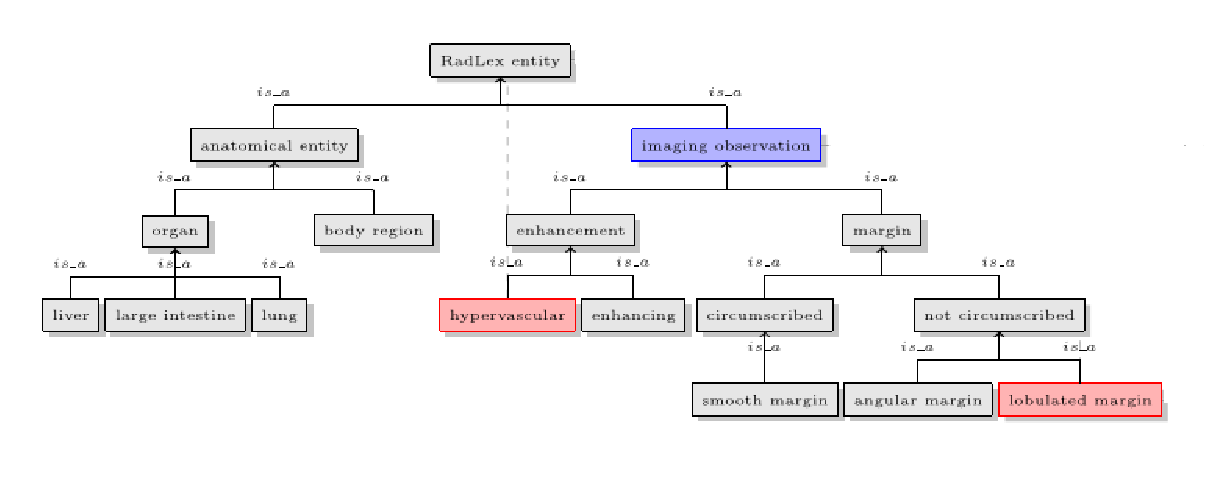
\includegraphics[width=1\columnwidth]{../figures/RadlexOnto}
\par\end{centering}
\fadaptada{Kurtz20141082}
\end{figure}

A fim de atingir nosso objetivo de classificar pacientes com câncer
é necessário representar um conhecimento geral do domínio \emph{(background
knowledge}). No caso deste trabalho, esse conhecimento é chamado \foreignlanguage{english}{\emph{sistema
de staging}}. No entanto, ter representações formais das definições
de um \foreignlanguage{english}{sistema de\emph{ staging}} numa ontologia
não é suficiente para fornecer ajuda automática na classificação de
tumores de câncer. Esse conhecimento deve ser representado também
em regras e axiomas (\foreignlanguage{english}{reasoning}). Portanto,
representar o conhecimento dos sistemas de \emph{staging} de cancer
como o TNM em ontologias e regras parece uma contribuição desejável
para a realização da classificação automática de tumores em imagens
médicas, e por conseguinte uma contribuição aos sistemas de apoio
à decisão auxiliada por computador. Os Conceitos como ontologias,
regras e \emph{reasoning} serão melhor detalhados no próximo capítulo. 

\subsection{Estágio do Câncer (\emph{Staging System})}

O estágio do câncer categoriza a progressão de um câncer no corpo,
em termos da extensão do tumor primário e de se espalhar para alguma
região próxima da origem do câncer. A rotina para determinar o estágio
de um câncer (\foreignlanguage{english}{\emph{cancer staging}}) em
pacientes tem uma série de vantagens reconhecidas por organizações
relacionadas a câncer em todo o mundo. O \foreignlanguage{english}{\emph{cancer
staging}} permite que os médicos possam determinar o tratamento mais
apropriadamente, avaliar os resultados de forma mais confiável e comparar
as estatísticas a nível local, regional e nacional com mais confiança
\citep{MCCOWAN2006}.

Esses benefícios têm motivado a criação de padrões internacionais
para \foreignlanguage{english}{\emph{cancer staging}}, como, por exemplo,
o padrão \emph{TNM} definido pela \emph{AJCC (}\foreignlanguage{english}{\emph{American
Joint Committee on Cancer}}\emph{)} e \emph{UICC (}\foreignlanguage{english}{\emph{International
Union Against Cancer}}\emph{).}

\subsection{O Padrão TNM}

O \emph{cancer st}aging no padrão \foreignlanguage{english}{TNM Classification
of Malignant Tumors} (TNM) é um processo de duas etapas. A primeira
etapa consiste em dar notas para três conceitos: descrição do tumor
(T), difusão em nós linfáticos (N) e possível metástase (M). Esses
conceitos estão resumidos na Tabela \ref{ResumodoprotocoloTNM}.

\begin{table}[h]
\caption{Os critérios de T, N e M para câncer de figado. \label{ResumodoprotocoloTNM}}

\noindent \begin{centering}
\begin{tabular}{>{\centering}p{0.15\columnwidth}>{\centering}p{0.06\columnwidth}>{\centering}m{0.7\columnwidth}}
\toprule 
\multirow{7}{0.15\columnwidth}{{\footnotesize{}T: }\foreignlanguage{english}{{\footnotesize{}Primary
Tumor}}{\footnotesize{} }} & {\footnotesize{}Tis} & \foreignlanguage{english}{{\footnotesize{}Primary tumor cannot be assessed}}\tabularnewline
\cmidrule{2-3} 
 & {\footnotesize{}T0} & \foreignlanguage{english}{{\footnotesize{}No evidence of primary tumor}}\tabularnewline
\cmidrule{2-3} 
 & {\footnotesize{}T1} & \foreignlanguage{english}{{\footnotesize{}Solitary tumor without vascular invasion}}\tabularnewline
\cmidrule{2-3} 
 & {\footnotesize{}T2} & \foreignlanguage{english}{{\footnotesize{}Solitary tumor with vascular invasion or multiple
tumors, none > 5 cm}}\tabularnewline
\cmidrule{2-3} 
 & {\footnotesize{}T3a} & \foreignlanguage{english}{{\footnotesize{}Multiple tumors > 5 cm}}\tabularnewline
\cmidrule{2-3} 
 & T3b & Single tumor or multiple tumors of any size involving a major branch
of the portal or hepatic vein\tabularnewline
\cmidrule{2-3} 
 & T4 & Tumor(s) with direct invasion of adjacent organs other than gallbladder
or with visceral peritoneum\tabularnewline
\midrule 
\multirow{3}{0.15\columnwidth}{{\footnotesize{}N: }\foreignlanguage{english}{{\footnotesize{}Regional
Lymph Node}}{\footnotesize{}s}} & NX & \foreignlanguage{english}{Regional lymph nodes cannot be assessed}\tabularnewline
\cmidrule{2-3} 
 & {\footnotesize{}N0} & \foreignlanguage{english}{{\footnotesize{}The cancer has not spread to lymph nodes. }}\tabularnewline
\cmidrule{2-3} 
 & {\footnotesize{}N1} & \foreignlanguage{english}{{\footnotesize{}The cancer has metastasized only to lymph nodes on
the same side as the cancerous liver.}}\tabularnewline
\midrule 
\multirow{2}{0.15\columnwidth}{{\footnotesize{}M: }\foreignlanguage{english}{{\footnotesize{}Distant
Metastasis}}} & {\footnotesize{}M0} & \foreignlanguage{english}{{\footnotesize{}The cancer has not spread to distant sites.}}\tabularnewline
\cmidrule{2-3} 
 & {\footnotesize{}M1} & \foreignlanguage{english}{{\footnotesize{}The cancer has spread to distant sites such as lymph
nodes farther than those mentioned in N stages, and other organs or
tissues such as the bones, or brain}}\tabularnewline
\bottomrule
\end{tabular}
\par\end{centering}
\fadaptada{Dameron2006Table}
\end{table}

A segunda etapa consiste na determinação do estagio de acordo com
as pontuações da fase anterior. As pontuações sobre T, N e M definem
um estágio único do tumor de 0 a IV. Note-se que várias combinações
de pontuações T, N e M podem levar ao mesmo estágio \citep{Dameron2006Table}.
Esses conceitos estão resumidos na Tabela \ref{stageTNM}.

\begin{table}[h]
\caption{Definições para os diferentes estágios de tumores.\label{stageTNM}}

\noindent \begin{centering}
\begin{tabular}{>{\centering}m{0.05\columnwidth}>{\centering}p{0.3\columnwidth}}
\toprule 
\foreignlanguage{english}{{\footnotesize{}Stage 0}} & {\footnotesize{}(Tis, N0, M0)}\tabularnewline
\midrule 
\foreignlanguage{english}{{\footnotesize{}Stage I}} & {\footnotesize{}(T1, N0, M0)}\tabularnewline
\midrule 
\foreignlanguage{english}{{\footnotesize{}Stage I}} & {\footnotesize{}(T2, N0, M0)}\tabularnewline
\midrule 
\foreignlanguage{english}{{\footnotesize{}Stage IIIA}} & {\footnotesize{}(T3a, N0, M0)}\tabularnewline
\midrule 
\foreignlanguage{english}{{\footnotesize{}Stage IIIB}} & \foreignlanguage{english}{{\footnotesize{}(T3b, N0, M0)}}\tabularnewline
\midrule 
StageIIIC & \foreignlanguage{english}{{\footnotesize{}(T4, N0, M0)}}\tabularnewline
\midrule 
\foreignlanguage{english}{{\footnotesize{}Stage IVA}} & \foreignlanguage{english}{{\footnotesize{}(Any T, any N, M1)}}\tabularnewline
\bottomrule
\end{tabular}
\par\end{centering}
\fadaptada{Dameron2006Table}
\end{table}


\section{Considerações Finais }

Recentemente pode ser visto que houve uma escalada da complexidade
na recolação dos dados médicos pelo fato dos avanços em tecnologias
relacionadas com aquisição de imagem. As novas tecnologias como dispositivos
médicos e sistemas de mediçao, geran grandes volumes de imagens como
tambem outros dados por paciente, e torna difícil para os médicos
analisar e fornecer diagnóstico ou prognósticos na hora. 

Este capítulo forneceu uma base teórica para compreensão de conceitos
como vocabulários controlados, anotações de imagem, anotação semântica
e representação do conhecimento. Foi mostrado também como esses conceitos
podem ser utilizados na área de informática biomédica para melhorar
processos como a interpretação de imagens médicas em câncer.
\end{document}
